\documentclass{article}

% if you need to pass options to natbib, use, e.g.:
% \PassOptionsToPackage{numbers, compress}{natbib}
% before loading nips_2017
%
% to avoid loading the natbib package, add option nonatbib:
% \usepackage[nonatbib]{nips_2017}

\usepackage{nips_2017}

% to compile a camera-ready version, add the [final] option, e.g.:
% \usepackage[final]{nips_2017}

\usepackage[utf8]{inputenc} % allow utf-8 input
\usepackage[T1]{fontenc}    % use 8-bit T1 fonts
\usepackage{hyperref}       % hyperlinks
\usepackage{url}            % simple URL typesetting
\usepackage{booktabs}       % professional-quality tables
\usepackage{amsfonts}       % blackboard math symbols
\usepackage{nicefrac}       % compact symbols for 1/2, etc.
\usepackage{microtype}      % microtypography
\usepackage{amsmath}
\usepackage{subcaption}
\usepackage{graphicx}
%\usepackage{subfigure}

\title{Generalised Off-line Training on\\ Spiking Deep Neural Networks}

% The \author macro works with any number of authors. There are two
% commands used to separate the names and addresses of multiple
% authors: \And and \AND.
%
% Using \And between authors leaves it to LaTeX to determine where to
% break the lines. Using \AND forces a line break at that point. So,
% if LaTeX puts 3 of 4 authors names on the first line, and the last
% on the second line, try using \AND instead of \And before the third
% author name.

\author{
  David S.~Hippocampus\thanks{Use footnote for providing further
    information about author (webpage, alternative
    address)---\emph{not} for acknowledging funding agencies.} \\
  Department of Computer Science\\
  Cranberry-Lemon University\\
  Pittsburgh, PA 15213 \\
  \texttt{hippo@cs.cranberry-lemon.edu} \\
  %% examples of more authors
  %% \And
  %% Coauthor \\
  %% Affiliation \\
  %% Address \\
  %% \texttt{email} \\
  %% \AND
  %% Coauthor \\
  %% Affiliation \\
  %% Address \\
  %% \texttt{email} \\
  %% \And
  %% Coauthor \\
  %% Affiliation \\
  %% Address \\
  %% \texttt{email} \\
  %% \And
  %% Coauthor \\
  %% Affiliation \\
  %% Address \\
  %% \texttt{email} \\
}

\begin{document}
% \nipsfinalcopy is no longer used

\maketitle

\begin{abstract}
  We extended the work of proposed activation function, Noisy Softplus, to fit into training of layered up deep spiking neural networks~(SNNs).
  Thus, a time-dependant, biologically-plausible spiking neuron can be modelled as a traditional rate-based neuron in artificial neural networks~(ANNs).
  Such an ANN can be trained simply by the traditional algorithm, for example Back Propagation~(BP), and the trained weights can be directly used in the spiking version of the same network without any conversion.
  Furthermore, the training method has been generalised to other activation units, for instance Rectified Linear Units (ReLU), to train deep SNNs off-line.
  This research is crucial to provide a generalised SNN training method, to improve the learning ability of SNNs with biological characteristics, and to close the gap towards equivalent performance as ANNs.
 
\end{abstract}

\section{Introduction}
DNNs are the most promising research field in computer vision, even exceeding human-level performance on image classification tasks~\cite{he2015delving}, and spiking DNNs offer the prospect of neuromorphic systems that combine remarkable performance with energy-efficient training and operation.Theoretical studies have shown that biologically-plausible learning, e.g. Spike-Timing-Dependent Plasticity (STDP), could approximate a stochastic version of powerful machine learning algorithms such as 
%	Expectation Maximization~\cite{nessler2013bayesian}, 
Contrastive Divergence~\cite{neftci2013event}, Markov Chain Monte Carlo~\cite{buesing2011neural} and Gradient Descent~\cite{o2016deep}.Yet, in practice, SNNs have not achieved the recognition/classification performance of their non-spiking competitor, and it remains an unsolved problem to develop SNNs with equivalent performance.

%How to map a well trained ANN to SNN is a hot topic in this field, especially using spiking neurons of biological scale.

On the  other  hand, the offline training of an ANN, which is then mapped to an SNN, has shown near loss-less conversion and state-of-the-art classification accuracy.
Jug et al\cite{Jug_etal_2012} first proposed the use of the Siegert function to replace the sigmoid activation function in training Restricted Boltzmann Machine (RBM).
The Siegert units map incoming currents driven by Poisson spike trains to the response firing rate of a Leaky Integrate-and-Fire (LIF) neuron.
The ratio of the spiking rate to its maximum is equivalent to the output of a sigmoid neuron.
A spiking Deep Belief Network (DBN)~\cite{Stromatias2015scalable} of four layers of RBMs was implemented on neuromorphic hardware, SpiNNaker~\cite{furber2014spinnaker}, to recognise hand written digits in real time.

Based on the fact that cortical neurons seldom saturate their firing rate as sigmoid neurons,ReLU~\cite{glorot2011deep} were proposed to replace sigmoid neurons and surpassed the performance of other popular activation units 
.
%trained with noisy input, the 4-layered spiking autoencoder reached 98.37\% accuracy on MNIST. 
Recent developments on ANN-trained SNN models has focused on using ReLU units and converting trained weights to fit in SNNs.
Better performance~\cite{cao2015spiking,diehl2015fast} than Siegert-trained RBM has been demonstrated in Spiking ConvNets, but this employed simple integrate and fire (IF) neurons without leakage.The training used only ReLUs and zero bias to avoid negative outputs, and applied a deep learning technique, dropout\cite{srivastava2014dropout} , to increase the classification accuracy.
Normalising the trained weights for use on an SNN employing IF neurons only was relatively straightforward and maintained classification accuracy.
This work was extended to a Recursive Neural Network (RNN)~\cite{diehl2016conversion} and run on the TrueNorth\cite{merolla2014million} neuromorphic hardware platform.

Except for the popular, simplified version of ReLU, $max(0,\sum w x)$, the other implementation of $\log(1+e^x)$, ``Softplus'', is more biologically realistic.
Recent work~\cite{hunsberger2015spiking} proposed the Soft LIF response function for training SNNs, which is equivalent to Softplus activation of ANNs. Furthermore, neuroscientific study has showed that the spike train of individual neurons is far from being periodic, which thus brings noisy to the input signal of spiking neurons~\cite{Gerstner:2002}. Therefore, in the previous work of Qian Liu et al.~\cite{Noisysoftplus}, the difference between analytical estimation and practical simulations of spiking neurons were compared, and a new activation function named Noisy Softplus was proposed to match the response function of LIF neurons. In order to close the gap between the performance of SNNs and ANNs, and to further improve the performance of SNNs, we extended Noisy Softplus with a scale factor and proposed a complete layered up SNN training method by using artificial neurons of combined activation.


\section{ANN-Trained SNNs}	

\subsection{Extended Noisy Softplus}
\label{sec:af_model}
Suppose $\lambda_{out}$ represents the firing rate  of a LIF neuron driven by a noisy current $x$, we extended Noisy Softplus\cite{Noisysoftplus} with a scale factor, $S$, then
\begin{equation}
\begin{aligned}
\lambda_{out} &\simeq f_{ns}(x, \sigma) \times S\\
&=k \sigma \log [1 + \exp(\frac{x}{k \sigma})] \times S.
\end{aligned}
\label{equ:fit}
\end{equation}	

Noisy Softplus fits well to the practical response firing rate of the LIF neuron with suitable calibration of $k$ and $S$, see Figure~\ref{Fig:nsptau1}.
The parameter pair of $(k, S)$ is curve-fitted with the triple data points of $(\lambda, x, \sigma)$.
The fitted parameter was set to $(k, S)=(0.19,208.76)$ for the practical response firing rate driven by synaptic noisy current with $\tau_{syn}=1$~ms and was set to $(k, S)=(0.35,201.06)$ when $\tau_{syn}=10$~ms.
The calibration currently is conducted by linear least squares regression; numerical analysis is considered however for future work to express the factors with biological parameters of a LIF neuron. From now on, we can model the response firing activity of a LIF neuron with a unified activation function, extended Noisy Softplus.

\begin{figure}
	\centering
	\begin{subfigure}[htb]{0.49\textwidth}
		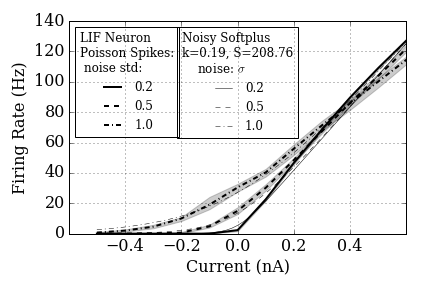
\includegraphics[width=\textwidth]{pics_iconip/4-1.png}
		\caption{$\tau_{syn}$=1~ms}
	\end{subfigure}
	\begin{subfigure}[htb]{0.49\textwidth}
		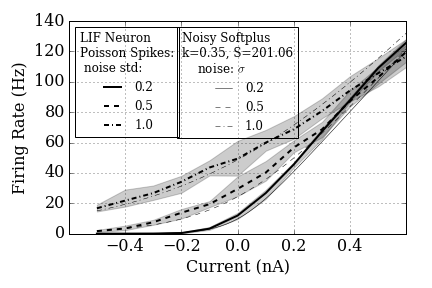
\includegraphics[width=\textwidth]{pics_iconip/4-10.png}
		\caption{$\tau_{syn}$=10~ms}
	\end{subfigure}
	\caption{Noisy Softplus fits to the response firing rates of LIF neurons.}
	\label{Fig:nsptau1}
\end{figure}		
In order to illustrate how we can use the extended Noisy Softplus to train layered up SNNs, we will demonstrate the mapping between the physical activity and numerical ANN calculations in the following subsections. 

\subsection{Equivalent Input and Output}

Neurons in ANNs take inputs from their previous layer, and feed the weighted sum of their input, $net_j = \sum_i w_{ij}x_i$, to the activation function.
The transformed signal then forms the output of an artificial neuron, which can be denoted as  $y_j=f(net_j)$.	
However, Noisy Softplus takes physical quantities of current, and firing rate as input/output, thus an extra step is still needed to map the firing rate to numerical values in ANNs.
According to Equation~\cite{Noisysoftplus}, the mean of the current feeding into a spiking neuron is equivalent to $net$ of artificial neurons, where
\begin{equation}
\begin{aligned}
& {m_I}_j = \sum_i w_{ij}(\lambda_{i}\tau_{syn})~, \textrm{  then}\\
& net_j= \sum_i w_{ij} x_i~~, \textrm{~~and~~}
x_i = \lambda_{i}\tau_{syn}~.
\end{aligned}
\label{equ:mi_input}
\end{equation}
The noise level of Noisy Softplus, $\sigma^2$, is the variance of the current, which also can be seen as a weighted sum of the same input $x$ but with different weights:
\begin{equation}
\begin{aligned}
& {s_I^2}_j=\sum_i(\frac{1}{2} w_{ij}^2) (\lambda_{i}\tau_{syn})~, \textrm{  then}\\
& \sigma^2_j= \sum_i (\frac{1}{2} w_{ij}^2) x_i~~.
\end{aligned}
\label{equ:si_input}
\end{equation}

\begin{figure}[bt!]
	\centering
	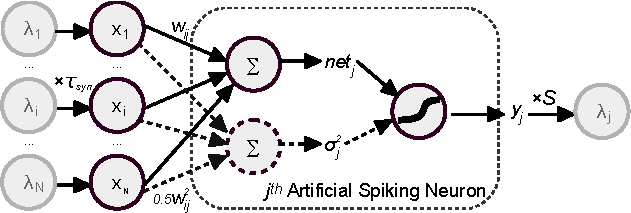
\includegraphics[width=0.8\textwidth]{pics_iconip/neuron_o.pdf}
	\caption{Artificial spiking neuron takes scaled firing rates as input, then transforms weighted sum in some activation unit to its output which can be scaled-up to the firing rate of an output spike train.}
	\label{Fig:sneuron}
\end{figure}

Noisy Softplus transforms the noisy current with parameters of $(net_j, \sigma_j)$ to the equivalent ANN output $y_j$ , where it can be scaled up by the factor $S$ to the firing rate of SNNs.
Note that the calculation of noise level is not necessary for activation functions other than Noisy Softplus, for example, it can be set to a constant for Softplus or 0 for ReLU.
We name the neuron model `artificial spiking neurons' which takes firing rates of spike trains as input and output. 
The entire artificial spiking neuron model is then generalised to any ReLU/Softplus-like activation functions, See Figure~\ref{Fig:sneuron}.


\subsection{Layered-up Network}
\label{subsec:ns_train}
%	Figure~\ref{Fig:sneuron} shows an complete transformation process of a spiking neuron, which mimics the biological neurons taking and generating spike trains.
Referred to Figure~\ref{Fig:sneuron}, if we move the left end process of $\times \tau_{syn}$ to the right end after $\lambda_j$, Figure~\ref{Fig:sneuron} forms the same neuron model and structure as multilayer perceptron: neurons take $x$ as input and outputs $y$, and this conversion is illustrated in Figure~\ref{Fig:tneuron}.
The process within such an artificial neuron is divided into weighted summation and activation, which also applies to SNN modelling by combining the scaling factor $S$ and the synaptic time constant $\tau_{syn}$ to activation functions.
Thus the combined activation function for modelling SNNs should be:
\begin{equation}
y = f(x) \times S \times \tau_{syn}~~,
\label{equ:full_act}
\end{equation}
and its derivative function which is used when back propagates is:
\begin{equation}
\frac{\partial y}{\partial x} = f'(x) \times S \times \tau_{syn}~~.
\end{equation}

\begin{figure}[tbh!]
	\centering
	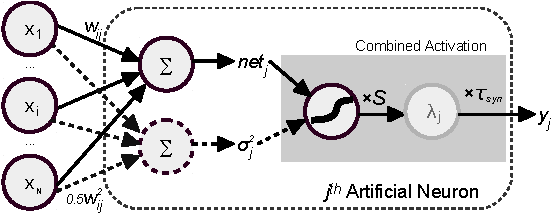
\includegraphics[width=0.8\textwidth]{pics_iconip/neuron_t.pdf}
	\caption{Transforming artificial spiking neurons to artificial neurons for SNN modelling. The combined activation links the firing activity of a spiking neuron to the numerical value of ANNs.}
	\label{Fig:tneuron}
\end{figure}


Thus, using this method of ANN-trained SNNs, the activation functions are of lower complexity than the Siegert formula, and their corresponding derivative functions can be directly used for back propagation.
Furthermore, the method enables ReLU-like activation functions for SNN training, thus improving the recognition accuracy while keeping a relative lower firing rate compared to sigmoid neurons. 
Most significantly, the ANN-trained weights are ready for use in SNNs without any transformation, and the output firing rate of a spiking neuron can be estimated in the ANN simulation.


\subsection{Fine Tuning}
There are two aspects to the fine tuning which makes the ANN closer to SNNs:
Firstly, using Noisy Softplus activation functions in a whole trained network operates every single neuron running in a similar noise level as in SNNs, thus the weights trained by other activation functions will be tuned to fit closer to SNNs.
Secondly, the output firing rate of any LIF neuron is greater than zero as long as noise exists in their synaptic input.
Thus adding up a small offset on the labels directs the model to approximate to practical SNNs. 

The labels of data are always converted to binary values for ANN training.
This enlarges the disparities between the correct recognition label and the rest to train the network for better classification capability.
Consequently, we can train the network with any activation function and then fine-tune it with Noisy Softplus to take account of both accuracy and practical network activities of SNNs.
However, we add a small number, for example 0.01, to all the binary values of the data labels.
Doing so helps the training to loosen the strict objective function to predict exact labels with binary values.
Instead, it allows a small offset to the objective.
An alternative method is to use Softmax function at the top layer, which aims to map real vectors to the range of $(0,1)$ that add up to 1. 
However, without a limit on the input of Softmax, it will be easy to reach or even exceed the highest firing rate of a spiking neuron.
The result of fine tuning on a Convnet will be demonstrated in subsection~\ref{subsec:result_compare}.


\section{Results}
\label{sec:iconipResult}
A convolutional network model was trained on MNIST,
%	~\cite{lecun1998gradient}
a popular database in neuromorphic vision, using the ANN-trained SNN method stated above.
The architecture contains $28\times28$ input units, followed by two convolutional layers 6c5-2s-12c5-2s, and 10 output neurons fully connected to the last pooling layer to represent the classified digit.

The training only employed Noisy Softplus units that all the convolution, average sampling, and the fully-connected neurons use Noisy Softplus function with no bias.
The parameters of the activation function were calibrated as, $(k=0.30, S=201)$,  for LIF neurons~($C_m =0.25$nF, $\tau_m =20.0$ms, $\tau_{refrac} =1.0$ms, $v_{reset} =-65.0$mV, $v_{rest} =-65.0$mV, $v_{thresh} =-50.0$mV, $i_{offset}= 0.1$nA, $\tau_{syn}=5$~ms).
The input images were scaled by 100~Hz to present the firing rates of input spikes.
The weights were updated using a decaying learning rate, 50 images per batch and 20 epochs.
The ANN-trained weights were then directly applied in the corresponding convolutional SNN without any conversion for recognition tasks.


\subsection{Neural Activity}
To validate how well the Noisy Softplus activation fits to the response firing rate of LIF neurons in a real application, we simulated the model on NEST using the Poisson MNIST dataset~\cite{liu2016bench} and the neurons of a convolutional map were observed.

A small test of ten MNIST digits presented in Poisson spike trains for 1~s each.
A trained $5\times5$ kernel was convolved with these input digits, and the convolved output of the feature map, the output firing rate was recorded during a real-time SNN simulation on NEST, and compared to the modelled activations of Equation~\ref{equ:full_act} in ANNs.

The input $x$ of the network was calculated as Equation~\ref{equ:mi_input}: $x_i=\lambda_i\tau_{syn}$, and so as the weighted sum of the synaptic current (see Equation~\ref{equ:mi_input}), $net_j$ and its variance (see Equation~\ref{equ:si_input}), $\sigma^2_j$.
With three combined activation functions as Equation~\ref{equ:full_act}:
\begin{equation}
\begin{aligned}
&\textrm{(1) Noisy Softplus:~~}  y_j=k \sigma_j \log [1 + \exp(\frac{net_j}{k \sigma_j})] \times S \times \tau_{syn}~~,  \\
&\textrm{(2) ReLU:~~ } y_j=max(0, net_j) \times S \times \tau_{syn}~~, \\
&\textrm{(3) Softplus:~~ } y_j=k \sigma \log [1 + \exp(\frac{net_j}{k \sigma})] \times S \times \tau_{syn}~~, ~~~\sigma=0.45,  
\end{aligned}
\end{equation}	
we compare the output to the recorded SNN simulations.
ReLU assumes a non-noise current, and Softplus takes a static noise level thus $\sigma_j$ is not used for either of them, meanwhile Noisy Softplus adapts to noise automatically with $\sigma_j$.
The experiment took the sequence of 10 digits to the same kernel and the estimated spike counts using Noisy Softplus fit to the real recorded firing rate much more accurately than ReLU and Softplus,  see~\ref{fig:af_compare}.
%	Figure~\ref{fig:af_stast} illustrated the statistics of error between the estimation and the recorded firing rate, $err = y_j - \lambda_j$ which formed normal distributions where Noisy Softplus hold the weakest mean (low in abstract) and lowest standard deviation.
The Euclidean distance, $\sqrt{\sum_{j}(y_j/\tau_{syn} - \lambda_j)}$, between the spike counts and the predicted firing rates by Noisy Softplus, ReLU and Softplus was 184.57, 361.64 and 1102.76 respectively.
We manually selected a static noise level of 0.45 for Softplus, whose estimated firing rates located roughly on the top slope of the real response activity.
This resulted in longer Euclidean distance than using ReLU, since most of the input noisy currents were of relatively low noise level in this experiment.
Hence, the firing rate driven by lower noise level is closer to ReLU curve than Softplus.

\begin{figure}[hb!]
	\centering
	\begin{subfigure}[hb]{0.32\textwidth}
		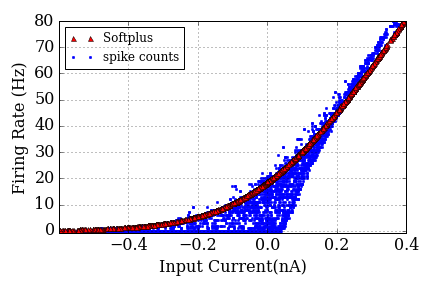
\includegraphics[width=\textwidth]{pics_iconip/6-5-1.png}
		\caption{Softplus}
	\end{subfigure}
	\begin{subfigure}[hb]{0.32\textwidth}
		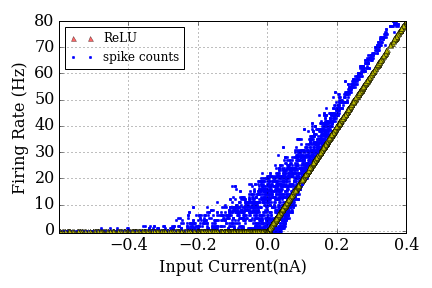
\includegraphics[width=\textwidth]{pics_iconip/6-5-2.png}
		\caption{ReLU}
	\end{subfigure}
	\begin{subfigure}[hb]{0.32\textwidth}
		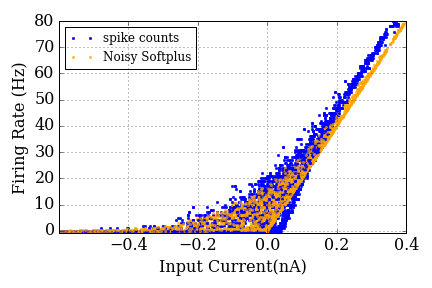
\includegraphics[width=\textwidth]{pics_iconip/6-5-3.png}
		\caption{Nosiy Softplus}
	\end{subfigure}
		\caption{Noisy Softplus fits to the neural response firing rate in an SNN simulation.
			The recorded firing rate of the same kernel convolved with 10 images in SNN simulation, comparing to the prediction of activations of Softplus, ReLU, and Noisy Softplus.}
		\label{fig:af_compare}
\end{figure}		

The SNN successfully classified the digits where the correct label neuron fired the most.
We trained the network with binary labels on the output layer, thus the expected firing rate of correct classification was $1/\tau_{syn}=200$~Hz according to Equation~\ref{Fig:tneuron}.
The firing rates of the recognition test fell to the valid range around 0 to 200~Hz.
This shows another advantage of the proposed ANN-trained method that we can constrain the expected firing rate of the top layer, thus preventing SNN from exceeding its maximum firing rate, for example 1000~Hz when time resolution of SNN simulation set to 1~ms.


\subsection{Recognition Performance}
\label{subsec:result_compare}
Here we focus on the recognition performance of the proposed ANN-trained SNN method.
Before looking into the recognition results, it is significant to see the learning capability of the proposed activation function, Noisy Softplus.
We compared the training using ReLU, Softplus, and Noisy Softplus by their loss during training averaged over 3 trials, see Figure~\ref{Fig:loss_ns}.
ReLU learned fastest with the lowest loss, thanks to its steepest derivative.
In comparison, Softplus accumulated spontaneous firing rates layer by layer and its derivative may experience vanishing gradients during back propagation, which result in a more difficult training.
Noisy Softplus performance lay between these two in terms of loss and learning speed.
However, the loss stabilised fastest, which means a possible shorter training time.
%\begin{figure}[tbp!]
%	\centering
%	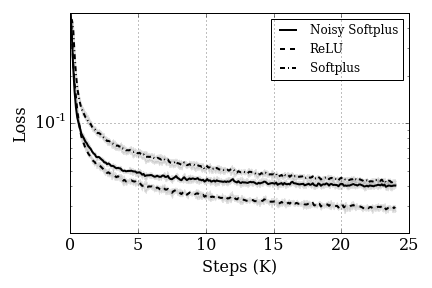
\includegraphics[width=0.7\textwidth]{pics_iconip/8.png}
%	\caption{Comparisons of Loss during training using Noisy Softplus, ReLU and Softplus activation functions. Bold lines show the average of three training trials, and the grey colour illustrates the range between the minimum and the maximum values of the trials.  }
%	\label{Fig:loss_ns}
%\end{figure}
%	The trained networks were scaled to SNNs and compared on recognition rates, 93.34\%, 96.43\% and 97.03\% with a conversion loss of 4.76\%, 0.91\% and 0.74\%.

\begin{figure}
	\begin{minipage}[t]{0.48\linewidth}
		\raggedleft
		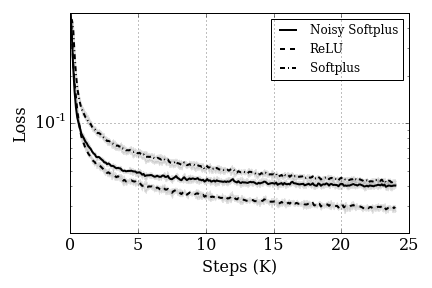
\includegraphics[width=2.6in]{pics_iconip/8.png}
		\caption{Comparisons of Loss during training using Noisy Softplus, ReLU and Softplus activation functions. Bold lines show the average of three training trials, and the grey colour illustrates the range between the minimum and the maximum values of the trials. }
		\label{Fig:loss_ns}
	\end{minipage}%
    \hspace{0.04\linewidth}
	\begin{minipage}[t]{0.48\linewidth}
		\raggedright
		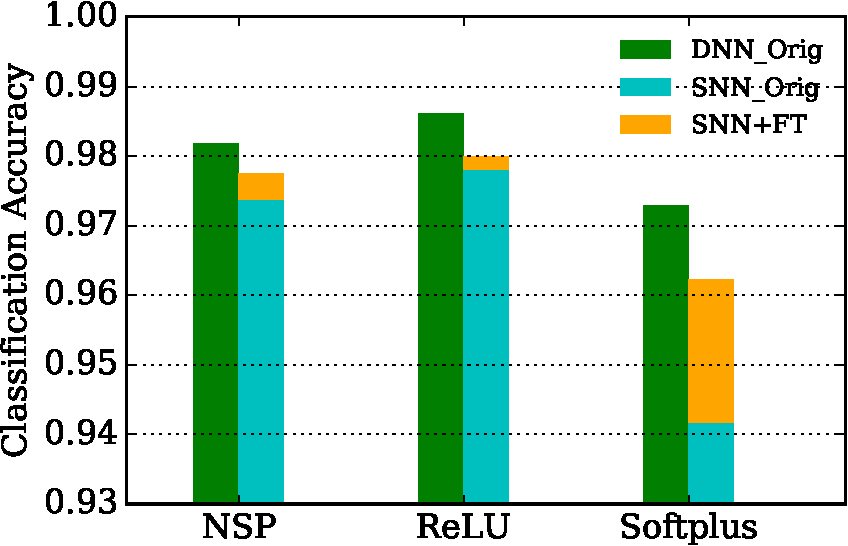
\includegraphics[width=2.6in]{pics_iconip/9-2.pdf}
		\caption{Classification accuracy compared among trained weights of Noisy Softplus, ReLU, Softplus on DNN, SNN and fine-tuned SNN.}
		\label{Fig:result_bar}
	\end{minipage}
\end{figure}

The recognition test took the whole testing dataset of MNIST which contains $10,000$ images.
At first, all trained models were tested on the same artificial neurons as used for training in ANNs, and these experiments were called `DNN' test since the network had a deep structure (5 layers).
Subsequently, the trained weights were directly applied to SNN without any transformation, and these `SNN' experiments tested their recognition performance on the NEST simulator.
The LIF neurons had the same parameters as in training.
The input images were converted to Poisson spike trains and presented for 1~s each.
The output neuron which fired the most indicated the classification of an input image.
Moreover, a `Fine tuning' test took the trained model for fine tuning, and the tuned weights were tested on the same SNN environment.
The tuning only ran for one epoch, 5\% cost of the ANN training (20~epochs), using Noisy Softplus neurons with labels shifted for $+0.01$.

The classification errors for the tests are investigated in Table~\ref{tbl:ns_result} and the averaged classification accuracy is shown in Figure~\ref{Fig:result_bar}.
From DNN to SNN, the classification accuracy declines by 0.80\%, 0.79\% and 3.12\% on average for Noisy softplus, ReLU and Softplus
The accuracy loss was caused by the mismatch between the activations and the practical response firing rates, see example in Figure~\ref{fig:af_compare}, and the strict binary labels for Noisy Softplus and Softplus activations.
Fortunately, the problem is alleviated by fine tuning which increased the classification accuracy by 0.38\%, 0.19\% and 2.06\%, and resulted in the total loss of 0.43\%, 0.61\%, and 1.06\% respectively.
The improvement of ReLU is not as great as the others, because there is no problem of strict labels during training.
%	Thus fine tuning mainly corrects the mismatch between ReLU and the firing rates in SNNs, and constraints the output firing rates of the network.
Softplus benefits the most from fine tuning, since not only the huge mismatch of response firing rate is greatly corrected, but also the offset on the labels helps the network to fit SNNs. 

%\begin{figure}[hbt!]
%	\centering
%	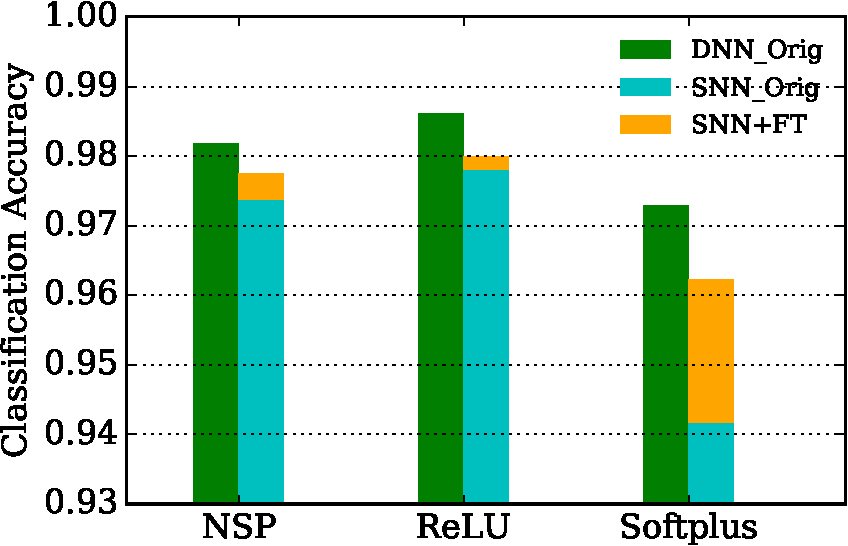
\includegraphics[width=0.7\textwidth]{pics_iconip/9-2.pdf}
%	\caption{Classification accuracy compared among trained weights of Noisy Softplus, ReLU, Softplus on DNN, SNN and fine-tuned SNN.}
%	\label{Fig:result_bar1}
%\end{figure}

\begin{table}[tbh] 
	\caption{Comparisons of classification accuracy (in \%) of ANN-trained convolutional neural models on original DNN, NEST simulated SNN, and SNN with fine-tuned (FT) model.}
	\begin{center}
		\bgroup
		\def\arraystretch{1.5}
		\begin{tabular} {r |c  c c |c c c |c c c}
			%First line
			\hline
			Trial No.
			&\multicolumn{3}{c|}{1} 
			&\multicolumn{3}{c|}{2}
			&\multicolumn{3}{c}{3}\\
			\hline
			Model
			& DNN & SNN &FT
			& DNN & SNN &FT
			& DNN & SNN &FT\\
			\hline
			\textbf{Noisy Sofplus}
			& 1.91 & 2.76 &2.45
			& 1.79 & 2.56 &2.19
			& 1.76 & 2.55 &2.10\\
			%				& 98.09 & 97.24 &97.55
			%				& 98.21 & 97.44 &97.81
			%				& 98.24 & 97.45 &97.90\\
			%				\hline
			\textbf{ReLU}
			& 1.36 & 2.03 &1.88
			& 1.46 & 2.28 &2.00
			& 1.36 & 2.25 &2.12\\
			%				& 98.64 & 97.97 &98.12
			%				& 98.54 & 97.72 &98.00
			%				& 98.64 & 97.75 &97.88\\
			%				\hline
			\textbf{Sofplus}
			& 2.30 & 5.66 &3.91
			& 2.75 & 5.22 &3.55
			& 2.42 & 6.62 &3.87\\
			%				& 97.70 & 94.34 &96.09
			%				& 97.25 & 94.78 &96.45
			%				& 97.58 & 93.38 &96.13\\
			\hline
		\end{tabular}
		\egroup
		\label{tbl:ns_result}
	\end{center}
\end{table}




%	The best classification accuracy achieved by SNNs was trained with ReLU and fine-tuned by Noisy Softplus.
The most efficient training in terms of both classification accuracy and algorithm complexity, takes ReLU for ANN training and Noisy Softplus for fine tuning.
Softplus does not exhibit better classification capability and more importantly the manual selected static noise level hugely influences the mismatch between the predicted firing rates and the real data.
Although Noisy Softplus shows the least classification drop from ANNs to SNNs, the training performance is still worse than ReLU.
%	Improved back propagation or other learning algorithms using noise level will be listed in the future work. 

The best classification accuracy achieved by SNN was 98.85\%, a 0.20\% drop from ANN test (99.05\%), which was trained with ReLU and fine-tuned by Noisy Softplus.
The network structure was the same with the state-of-the-art model which reported the best classification accuracy of 99.1\%~\cite{diehl2015fast} in ANN-trained SNNs: 12c5-2s-64c5-2s-10fc.
Their nearly loss-less conversion from ANNs to SNNs was achieved by using IF neurons, while our network performs the best among SNNs consisted of LIF neurons to our knowledge.

\begin{figure}[htb!]
	\centering
	\begin{subfigure}[t]{0.49\textwidth}
		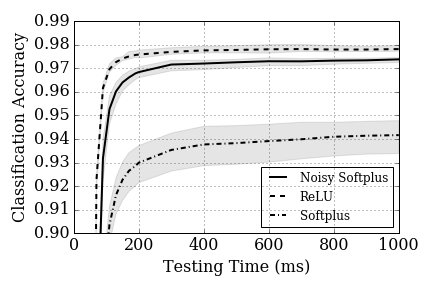
\includegraphics[width=\textwidth]{pics_iconip/8-2.png}
		\caption{Before fine tuning}
	\end{subfigure}
	\begin{subfigure}[t]{0.49\textwidth}
		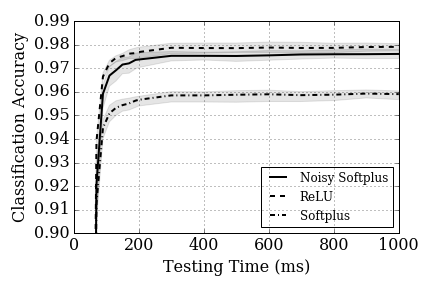
\includegraphics[width=\textwidth]{pics_iconip/8-3.png}
		\caption{After fine tuning.}
	\end{subfigure}
	
	\caption{The classification accuracy of 3 trials (averaged in bold lines, grey shading shows the range between minimum to maximum) over short response times, with (a) trained weights before fine tuning, and (b) after fine tuning.}
	\label{fig:ca_time}	
\end{figure}

As it is a major concern in neuromorphic vision, the recognition performance over short response times is also estimated in Figure~\ref{fig:ca_time}.
After fine tuning, Softplus significantly reduced the mismatch since the randomness among the three trials shrinks to a range similar to other experiments.
More obviously, fine tuning improved its classification accuracy and the response latency.
Notice that all of the networks trained by three different activation functions showed a very similar stabilisation curve against time, which means they all reached an accuracy close to their best by only taking 300~ms of test. 


\subsection{Power Consumption}
Noisy Softplus can easily be used for energy cost estimation for SNNs.
For a single neuron, the energy consumption of the synaptic events it triggers is:
\begin{equation}
\begin{aligned}
E_{j} &= \lambda_j N_j T E_{syn}\\
&= \dfrac{y_j N_j T E_{syn}}{\tau_{syn}}~~,
\end{aligned}
\label{equ:energy}
\end{equation}
where $\lambda_j$ is the output firing rate, $N_j$ is the number of post-synaptic neurons it connects to, $T$ is the testing time, and $E_{syn}$ is the energy cost for a synaptic event of some specific neuromorphic hardware, for example, about 8~nJ on SpiNNaker~\cite{stromatias2013power}.
Thus to estimate the whole network, we can sum up all the synaptic events of all the neurons:
\begin{equation}
\sum_j E_{j} =  \dfrac{T E_{syn}}{\tau_{syn}} \sum_{j}y_j N_j.
\end{equation}
Thus, it may cost SpiNNaker 0.064~W, 192~J running for $3,000$~s with synaptic events of $8\times10^6/s$ to classify $10,000$ images (300~ms each) with an accuracy of 98.02\%.
The best performance reported using the larger network may cost SpiNNaker 0.43~W operating synaptic event rate at $5.34\times10^7/s$, consume 4271.6~J to classify all the images for 1~s each.

\section{Discussions}
	Most significantly, we proposed the Noisy Softplus activation function which accurately models response firing rate of LIF neurons and overcomes the drawbacks of Siegert units.
\begin{itemize}
	\item Noisy Softplus takes account of time correlation of the noisy synaptic current, e.g. $\tau_{syn}$, which fits more to the actual response firing rate.
	
	\item Noisy Softplus can be applied easily to any training method, for example BP, thanks to its differentiability.
	
	\item the calculation on Noisy Softplus is no more than Softplus function, except for doubled computation on weighted sum of its input ($net$ and $\sigma$ in Equations~\ref{equ:mi_input} and~\ref{equ:si_input}), which is much more simplified than Siergert function.
	
	\item as one of the ReLU-liked activation function, the output firing rate seldom exceed the working range of a LIF neuron, for example the firing rates were around 0-200~Hz in the ConvNet model.
	
	\item the learning performance of Noisy Softplus is between Softplus and ReLU, which is supposed to outperform most of the other popular activation functions: for instance sigmoid.
\end{itemize}
Moreover, we proposed complete SNN modelling method by using artificial neurons of combined activation;
this method can be generalised to activation units other than Noisy Softplus.
The training of an SNN model is exactly the same as ANN training, and the trained weights can be directly used in SNN without any transformation.
This method is simpler and even more straight-forward than the other ANN offline training methods which requires an extra step of converting ANN-trained weights to SNN's.

In terms of classification/recognition accuracy, the performance of ANN-trained SNNs is nearly equivalent as ANNs, and the performance loss can  be partially solved by fine tuning.
The best classification accuracy of 98.85\% using LIF neurons in PyNN simulation outperforms state-of-the-art SNN models of LIF neurons which will be listed in Chapter~6, and is very close to the result using IF neurons~\cite{diehl2015fast}.

\section*{Acknowledgments}
To be added after reviewing.
%The work presented in this paper was largely inspired by discussions at the 2015 Workshops on Neuromorphic Cognition Engineering in CapoCaccia.The authors would like to thank the organisers and the sponsors.The authors would also like to thank Patrick Camilleri, Michael Hopkins, and Viv Woods for meaningful discussions and proof-reading the paper.The construction of the SpiNNaker machine was supported by the Engineering and Physical Sciences Research Council (EPSRC grant EP/4015740/1) with additional support from industry partners ARM Ltd and Silistix Ltd.The research leading to these results has received funding from the European Research Council under the European Union's Seventh Framework Programme (FP/2007-2013) / ERC Grant Agreement n. 320689 and from the EU Flagship Human Brain Project (FP7-604102). The research leading to these results has received funding from Natural Science Foundation of Guangdong Province, China (No: 2016A030313713) and also from  Natural Science Foundation of Guangdong Province, China (No: 2014A030310169).

%The research leading to these results has received funding from the European Research Council 
%(FP/2007-2013) / ERC Grant Agreement n. 320689 and from the EU Flagship Human Brain Project (FP7-604102). 
%Yunhua Chen received funding from the Natural Science Foundation of Guangdong Province, China (No: 2016A030313713) and also from  the Natural Science Foundation of Guangdong Province, China (No: 2014A030310169).
%Qian Liu personally thanks to the funding from the National Natural Science Foundation of China (61662013,U1501252), the Guangxi Natural Science Foundation~(2014GXNSFDA118036), and The High Level of Innovation Team of Colleges and Universities in Guangxi and Outstanding Scholars Program Funding.

\small

\bibliographystyle{unsrt}
\bibliography{ref}
\end{document}
